\documentclass[10pt,a4paper]{article}

% ------------------------------------------------------------------------------
% Typography & Reading Comfort (XeLaTeX + Native OpenType/TrueType Fonts)
% ------------------------------------------------------------------------------
\usepackage{fontspec}
\setmainfont{Source Sans 3}[
    UprightFont = *,
    BoldFont = * Bold,
    ItalicFont = * Italic,
    Scale = 1.0
]
\setmonofont{Roboto Mono}[Scale=0.86]
\usepackage{microtype}
\usepackage{setspace}
\setstretch{1.20}

\usepackage[margin=0.82in,top=0.92in,bottom=0.88in,headheight=20pt]{geometry}
\usepackage{xcolor}
\usepackage{graphicx}
\usepackage{tikz}
\usetikzlibrary{arrows.meta,positioning,shapes.geometric,fit,backgrounds,calc}
\usepackage{pgfplots}
\pgfplotsset{compat=1.18}
\usepackage[most]{tcolorbox}
\usepackage{booktabs}
\usepackage{tabularx}
\usepackage{array}
\usepackage{enumitem}
\usepackage{fancyhdr}
\usepackage{titlesec}
\usepackage{xurl}
\usepackage{hyperref}
\usepackage{float}

% ------------------------------------------------------------------------------
% Restrained Editorial Color Palette (Paper White, Charcoal Ink, Navy & Teal)
% ------------------------------------------------------------------------------
\definecolor{HeadingInk}{HTML}{111827}
\definecolor{BodyInk}{HTML}{374151}
\definecolor{MutedInk}{HTML}{6B7280}
\definecolor{NavyPrimary}{HTML}{1E3A5F}
\definecolor{TealAccent}{HTML}{0F766E}
\definecolor{AmberNote}{HTML}{92400E}
\definecolor{SurfaceTint}{HTML}{F8FAFC}
\definecolor{NavyTint}{HTML}{F1F5F9}
\definecolor{TealTint}{HTML}{F0FDFA}
\definecolor{BorderGray}{HTML}{CBD5E1}
\definecolor{LightRule}{HTML}{E5E7EB}

\hypersetup{
    colorlinks=true,
    linkcolor=NavyPrimary,
    urlcolor=NavyPrimary,
    pdftitle={Neutron v3.0 - System Architecture and Technical Specification},
    pdfauthor={Md Fahim Sarker}
}

% ------------------------------------------------------------------------------
% Page Headers, Footers & Section Styling
% ------------------------------------------------------------------------------
\pagestyle{fancy}
\fancyhf{}
\renewcommand{\headrulewidth}{0.4pt}
\renewcommand{\headrule}{\hbox to\headwidth{\color{LightRule}\leaders\hrule height \headrulewidth\hfill}}
\renewcommand{\footrulewidth}{0.4pt}
\renewcommand{\footrule}{\hbox to\headwidth{\color{LightRule}\leaders\hrule height \footrulewidth\hfill}}

\fancyhead[L]{\fontsize{8}{10}\selectfont\color{MutedInk}Neutron v3.0 \textemdash{} System Architecture Specification}
\fancyhead[R]{\fontsize{8}{10}\selectfont\color{MutedInk}Technical Reference}
\fancyfoot[L]{\fontsize{8}{10}\selectfont\color{MutedInk}github.com/fahiiim/Neutron-Web-Crawler}
\fancyfoot[R]{\fontsize{8}{10}\selectfont\color{HeadingInk}\thepage}

\titleformat{\section}
  {\Large\bfseries\color{HeadingInk}}
  {\color{NavyPrimary}\thesection.}
  {0.6em}
  {}
  [\vspace{3pt}{\color{LightRule}\titlerule[0.8pt]}]

\titleformat{\subsection}
  {\large\bfseries\color{NavyPrimary}}
  {\thesubsection}
  {0.55em}
  {}

\titleformat{\subsubsection}
  {\normalsize\bfseries\color{HeadingInk}}
  {\thesubsubsection}
  {0.5em}
  {}

\setlength{\parskip}{0.55em}
\setlength{\parindent}{0pt}

% Subtle left-accent editorial note box (minimalist, zero drop shadow)
\newtcolorbox{designnote}[1][]{
    enhanced,
    breakable,
    colback=SurfaceTint,
    colframe=SurfaceTint,
    borderline west={2.2pt}{0pt}{NavyPrimary},
    boxrule=0pt,
    arc=0pt,
    left=10pt, right=10pt, top=7pt, bottom=7pt,
    before upper={\ifstrempty{#1}{}{\textbf{\color{NavyPrimary}#1}\par\vspace{2pt}}}
}

\newcommand{\logoicon}[2][15pt]{\includegraphics[height=#1]{assets/logos/#2.png}}

% ------------------------------------------------------------------------------
% Document Body
% ------------------------------------------------------------------------------
\begin{document}
\color{BodyInk}
\sloppy

% ==============================================================================
% CLEAN EDITORIAL COVER PAGE (Light Paper, Structured Metadata, Subtle Accents)
% ==============================================================================
\begin{titlepage}
\thispagestyle{empty}
\begin{tikzpicture}[remember picture, overlay]
    \fill[NavyPrimary] (current page.north west) rectangle ($(current page.north east)+(0,-0.22cm)$);
    \fill[TealAccent] ($(current page.north west)+(0,-0.22cm)$) rectangle ($(current page.north east)+(0,-0.30cm)$);
\end{tikzpicture}

\vspace*{0.4cm}
{\fontsize{9.5}{12}\selectfont\bfseries\color{TealAccent} SYSTEM DESIGN \& ARCHITECTURE SPECIFICATION}

\vspace{0.2cm}
{\fontsize{28}{33}\selectfont\bfseries\color{HeadingInk} Neutron Search Engine\\\& Distributed Web Crawler}

\vspace{0.25cm}
{\fontsize{12.5}{17}\selectfont\color{MutedInk} Version 3.0 \textemdash{} High-Level Design, Low-Level Internals, and Cloud Infrastructure}

\vspace{0.45cm}
\noindent\rule{\textwidth}{0.6pt}
\vspace{0.3cm}

\textbf{\color{HeadingInk}Abstract}\\[0.2em]
Neutron is a privacy-focused web search engine, on-demand crawler, and citation synthesis system structured around three decoupled Python microservices communicating over ConnectRPC/Protobuf, a serverless Turso (LibSQL) FTS5 index, and a static React web client. This specification documents the deployed v3.0 architecture across GitHub Pages and Render Free instances, detailing request routing, hybrid cache-first and server-streaming crawl execution, lexical query normalization and ranking, HTML extraction, bounded deduplication, and storage modeling.

\vspace{0.35cm}
\renewcommand{\arraystretch}{1.28}
\noindent\begin{tabular}{@{}p{3.6cm} l@{}}
\toprule
\multicolumn{2}{@{}l}{\textbf{\color{HeadingInk}Document Metadata}} \\
\midrule
\textcolor{MutedInk}{Author} & Md Fahim Sarker \\
\textcolor{MutedInk}{System Release} & Neutron v3.0 (\texttt{main}) \\
\textcolor{MutedInk}{Runtime} & Python 3.12.8 (FastAPI, ConnectRPC) / React 18 (TypeScript, Vite) \\
\textcolor{MutedInk}{Primary Storage} & Turso LibSQL (SQLite FTS5 + Zstandard level-3 BLOBs) \\
\textcolor{MutedInk}{Hosting Platforms} & GitHub Pages (Frontend) · Render Free, Oregon (3 Web Services) \\
\textcolor{MutedInk}{Source Repository} & \url{https://github.com/fahiiim/Neutron-Web-Crawler} \\
\textcolor{MutedInk}{Public Gateway} & \url{https://neutron-gateway.onrender.com} \\
\bottomrule
\end{tabular}

\vspace{0.45cm}
\textbf{\color{HeadingInk}Core Technology Stack}
\vspace{0.3em}

\begin{tcolorbox}[enhanced, colback=SurfaceTint, colframe=LightRule, boxrule=0.6pt, arc=3pt, left=10pt, right=10pt, top=8pt, bottom=8pt]
\centering
\renewcommand{\arraystretch}{1.3}
\begin{tabular}{cccccc}
\logoicon[18pt]{react} & \logoicon[18pt]{typescript} & \logoicon[18pt]{vite} & \logoicon[18pt]{tailwindcss} & \logoicon[18pt]{fastapi} & \logoicon[18pt]{python} \\
{\scriptsize React 18} & {\scriptsize TypeScript} & {\scriptsize Vite 6} & {\scriptsize Tailwind v4} & {\scriptsize FastAPI} & {\scriptsize Python 3.12} \\[4pt]
\logoicon[18pt]{connectrpc} & \logoicon[18pt]{turso} & \logoicon[18pt]{sqlite} & \logoicon[18pt]{render} & \logoicon[18pt]{github} & \logoicon[18pt]{gemini} \\
{\scriptsize ConnectRPC} & {\scriptsize Turso LibSQL} & {\scriptsize SQLite FTS5} & {\scriptsize Render} & {\scriptsize GitHub Pages} & {\scriptsize Gemini 2.5} \\
\end{tabular}
\end{tcolorbox}

\vfill
\noindent\rule{\textwidth}{0.4pt}\\[0.2em]
{\footnotesize\color{MutedInk}Document derived strictly from verified production source files in \texttt{services/}, \texttt{spaces/crawler/}, \texttt{proto/}, \texttt{migrations/}, and \texttt{frontend/}.}
\end{titlepage}

% ==============================================================================
% TABLE OF CONTENTS & SECTION 1
% ==============================================================================
\tableofcontents
\vspace{0.6em}
\noindent\rule{\textwidth}{0.5pt}

\section{System Overview \& Architectural Goals}

Search engines deployed on low-cost or serverless infrastructure face two competing constraints: full-text database lookups are fast (tens of milliseconds) but limited to previously indexed pages, whereas live multi-source web crawling yields fresh coverage at the cost of network latency, anti-bot blocking, and higher CPU/memory usage.

Neutron resolves this trade-off through an adaptive two-tier retrieval design backed by strict service separation:
\begin{itemize}[leftmargin=1.4em, itemsep=3pt]
    \item \textbf{Edge Separation:} Presentation assets live on GitHub Pages while public API orchestration (\texttt{services/gateway}), index query/synthesis (\texttt{services/search}), and live web crawling (\texttt{services/crawler}) run as isolated Render web services bound by Protobuf v3 contracts (\texttt{proto/neutron/v1/neutron.proto}).
    \item \textbf{Cache-First, Stream-Second Execution:} Queries meeting \texttt{JIT\_CACHE\_THRESHOLD} (\texttt{5} indexed matches) return immediately from Turso FTS5 (or Gateway's \texttt{300\,s} \texttt{\_TTLCache}). Sparse or refreshed queries trigger \texttt{CrawlerService.StreamCrawl}, pushing real-time discovery and crawl updates to the browser over Server-Sent Events (SSE).
    \item \textbf{Predictable Free-Tier Resource Bounds:} Shared \texttt{0.1\,vCPU} / \texttt{512\,MB} worker limits are respected through \texttt{12\,KB} SimHash truncation, an \texttt{80}-link extraction cap per document, bounded async semaphores (\texttt{MAX\_CONCURRENT\_JIT\_FETCHES = 12}), and explicit \texttt{8.5\,s} batch deadlines.
    \item \textbf{Minimalist Data Retention:} The system sets no cookies, logs no client IP addresses to disk, validates external links via \texttt{safeHttpUrl}, and renders reader Markdown strictly through \texttt{marked} and \texttt{DOMPurify}.
\end{itemize}

\begin{table}[H]
\centering
\small
\renewcommand{\arraystretch}{1.28}
\begin{tabularx}{\textwidth}{@{}p{3.4cm} >{\ttfamily\scriptsize\raggedright\arraybackslash}p{4.1cm} >{\raggedright\arraybackslash}X@{}}
\toprule
\textbf{Service / Layer} & \textbf{Primary Entrypoint} & \textbf{Core Responsibility} \\
\midrule
Static Web Client & frontend/src/App.tsx & Search UI, \texttt{sessionStorage} cache (5\,m), SSE event consumer, Markdown reader modal, and Architecture view. \\
Edge Gateway & services/gateway/app.py & REST/SSE/ConnectRPC coordinator, \texttt{\_TTLCache}, \texttt{slowapi} rate limits, \texttt{X-Request-Id} propagation, and cold-start wake pings. \\
Search Service & services/search/app.py & ConnectRPC \texttt{SearchService}: wide-pool FTS5 queries, re-ranking, Zstd payload decompression, and Gemini/extractive synthesis. \\
Crawler Service & services/crawler/app.py & ConnectRPC \texttt{CrawlerService}: 6 parallel discovery sources, \texttt{StreamCrawl}, \texttt{robots.txt} cache, \texttt{curl\_cffi} fetch, and Bloom/SimHash dedup. \\
Storage Engine & migrations/03\_turso\_fts5\_schema.sql & Single Turso LibSQL database storing index metadata, Porter \texttt{FTS5} triggers, Zstd BLOBs, frontier tasks, and hot topics. \\
\bottomrule
\end{tabularx}
\caption{Service responsibilities across the Neutron v3.0 codebase.}
\end{table}

% ==============================================================================
% SECTION 2: CLOUD ARCHITECTURE
% ==============================================================================
\clearpage
\section{Cloud Architecture \& Network Topology}

Figure~\ref{fig:cloud-arch} shows the production deployment layout across GitHub, Render (Oregon), Turso, Google Gemini, and external web sources. Because Render Free web services do not expose private mesh networking across separate free instances, \texttt{neutron-gateway} communicates with \texttt{neutron-search} and \texttt{neutron-crawler} over public HTTPS using \texttt{pyqwest.HTTPTransport} configured with \texttt{certifi} root certificates and shared Bearer authentication (\texttt{INTERNAL\_API\_KEY}).

\begin{figure}[H]
\centering
\resizebox{0.97\textwidth}{!}{\begin{tikzpicture}[
    node distance=1.1cm and 1.1cm,
    cnode/.style={
        rectangle, rounded corners=3pt, draw=#1, fill=white,
        line width=0.75pt, inner sep=7pt, text width=3.9cm, align=center
    },
    zone/.style={
        rectangle, rounded corners=4pt, draw=BorderGray, dashed, fill=SurfaceTint,
        line width=0.7pt, inner xsep=14pt, inner ysep=16pt
    },
    arr/.style={-{Stealth[length=2.2mm]}, line width=0.8pt, draw=NavyPrimary},
    darr/.style={-{Stealth[length=2.1mm]}, dashed, line width=0.75pt, draw=MutedInk}
]

% Row 1: Client & CDN
\node[cnode=NavyPrimary] (browser) {
    \logoicon[13pt]{react}\;\logoicon[13pt]{typescript}\;\logoicon[13pt]{vite}\\[3pt]
    \textbf{\small Browser Client (SPA)}\\
    {\scriptsize React 18 · Tailwind v4 · DOMPurify\\5-min \texttt{sessionStorage} Cache}
};

\node[cnode=BorderGray, right=1.8cm of browser] (ghpages) {
    \logoicon[13pt]{githubpages}\;\logoicon[13pt]{githubactions}\\[3pt]
    \textbf{\small GitHub Pages \& Actions}\\
    {\scriptsize \texttt{deploy\_pages.yml} · \texttt{ci\_cd.yml}\\Preconnect TLS · Static Assets}
};

% Row 2: Gateway
\node[cnode=NavyPrimary, below=1.95cm of $(browser)!0.5!(ghpages)$, text width=4.8cm] (gateway) {
    \logoicon[13pt]{render}\;\logoicon[13pt]{fastapi}\;\logoicon[13pt]{connectrpc}\\[3pt]
    \textbf{\small \texttt{neutron-gateway} (Render Free)}\\
    {\scriptsize REST · SSE \texttt{/search/stream} · \texttt{GatewayService}\\\texttt{\_TTLCache} (300\,s) · \texttt{slowapi} · \texttt{X-Request-Id}}
};

% Row 3: Search & Crawler
\node[cnode=TealAccent, below left=1.35cm and 0.35cm of gateway, text width=4.3cm] (searchsvc) {
    \logoicon[13pt]{fastapi}\;\logoicon[13pt]{python}\;\logoicon[13pt]{connectrpc}\\[3pt]
    \textbf{\small \texttt{neutron-search} (Render Free)}\\
    {\scriptsize \texttt{SearchService} (ConnectRPC)\\FTS5 Query · Re-ranking · Reader\\Gemini + Extractive Synthesis}
};

\node[cnode=TealAccent, below right=1.35cm and 0.35cm of gateway, text width=4.3cm] (crawlersvc) {
    \logoicon[13pt]{fastapi}\;\logoicon[13pt]{curl}\;\logoicon[13pt]{connectrpc}\\[3pt]
    \textbf{\small \texttt{neutron-crawler} (Render Free)}\\
    {\scriptsize \texttt{CrawlerService} (\texttt{StreamCrawl})\\6 Parallel Adapters · Chrome 124 TLS\\1M Bloom Filter · 12\,KB SimHash}
};

% Row 4: Data & External Services
\node[cnode=NavyPrimary, below=1.4cm of searchsvc, text width=4.3cm] (turso) {
    \logoicon[13pt]{turso}\;\logoicon[13pt]{sqlite}\\[3pt]
    \textbf{\small Turso LibSQL (Serverless)}\\
    {\scriptsize \texttt{search\_index} · \texttt{search\_fts} (Porter)\\\texttt{page\_payloads} (Zstd L3) · \texttt{hot\_topics}}
};

\node[cnode=BorderGray, left=0.9cm of turso, text width=3.3cm] (gemini) {
    \logoicon[13pt]{gemini}\\[3pt]
    \textbf{\small Gemini 2.5 Flash}\\
    {\scriptsize Optional REST API\\4.5\,s Timeout · Citations}
};

\node[cnode=NavyPrimary, below=1.4cm of crawlersvc, text width=4.3cm] (web) {
    \logoicon[12pt]{duckduckgo}\;\logoicon[12pt]{wikipedia}\;\logoicon[12pt]{arxiv}\;\logoicon[12pt]{github}\;\logoicon[12pt]{reddit}\;\logoicon[12pt]{hackernews}\\[3pt]
    \textbf{\small Open Web \& Discovery APIs}\\
    {\scriptsize DDG · Wikipedia · arXiv · GitHub · Reddit · HN\\\texttt{robots.txt} Enforced · Domain Diversity}
};

% Background Render Cluster Boundary
\begin{scope}[on background layer]
    \node[zone, fit=(gateway)(searchsvc)(crawlersvc)] (rzone) {};
    \node[anchor=north east, font=\scriptsize\bfseries\color{MutedInk}, inner sep=5pt] at (rzone.north east) {Render Free Web Services (Oregon · Python 3.12.8)};
\end{scope}

% Edges
\draw[darr] (ghpages) -- node[above, font=\scriptsize\color{MutedInk}] {Static Bundle} (browser);
\draw[arr] (browser.south) |- ++(0,-0.40cm) -| node[pos=0.25, above, font=\scriptsize\bfseries\color{NavyPrimary}] {HTTPS JSON / SSE} (gateway.north);
\draw[arr] (gateway.south west) -- node[left, font=\scriptsize, align=right, color=BodyInk] {ConnectRPC / HTTPS\\Bearer + \texttt{X-Request-Id}} (searchsvc.north);
\draw[arr, color=TealAccent] (gateway.south east) -- node[right, font=\scriptsize, align=left, color=BodyInk] {\texttt{StreamCrawl} Stream\\55\,s RPC Timeout} (crawlersvc.north);
\draw[arr] (searchsvc.south) -- node[left, font=\scriptsize, color=MutedInk] {\texttt{libsql-client}} (turso.north);
\draw[arr] (crawlersvc.south west) -- node[above left, font=\scriptsize, color=MutedInk] {Batch Upsert} (turso.north east);
\draw[darr] (searchsvc.west) -| node[above, near start, font=\scriptsize, color=MutedInk] {REST (Optional)} (gemini.north);
\draw[arr, color=TealAccent] (crawlersvc.south) -- node[right, font=\scriptsize, color=MutedInk] {\texttt{httpx} + \texttt{curl\_cffi}} (web.north);

\end{tikzpicture}}
\caption{Cloud infrastructure and inter-service communication boundaries.}
\label{fig:cloud-arch}
\end{figure}

\subsection{Cold-Start \& Cross-Origin Resilience}
Free-tier Render services sleep after 15 minutes of inactivity and require roughly 30--50 seconds to cold-boot:
\begin{itemize}[leftmargin=1.4em, itemsep=2pt]
    \item \textbf{Auto-Resolved Blueprint URLs:} In \texttt{services/common/config.py}, when \texttt{RENDER=true} and local overrides are unset, \texttt{GatewayServiceSettings} defaults to the public \texttt{.onrender.com} hostnames.
    \item \textbf{Throttled Warm-Up Pings:} \texttt{\_maybe\_wake\_downstream()} issues background \texttt{/health} requests (throttled to at most once every \texttt{180\,s}) to both \texttt{neutron-search} and \texttt{neutron-crawler} on \texttt{/health}, \texttt{/stats}, or downstream \texttt{502}/\texttt{503} failures.
    \item \textbf{Preconnect \& Timeout Envelope:} \texttt{frontend/index.html} declares \texttt{<link rel="preconnect">} to \texttt{neutron-gateway.onrender.com}, while \texttt{RPC\_TIMEOUT\_MS=55000} spans cold container boots. Custom \texttt{429} and \texttt{500} FastAPI exception handlers ensure CORS headers remain attached when downstream calls fail.
\end{itemize}

% ==============================================================================
% SECTION 3: HIGH-LEVEL DESIGN (HLD)
% ==============================================================================
\section{High-Level Design (HLD): Request Lifecycle \& Streaming}

Every search query enters either \texttt{/search} (JSON), \texttt{/api/research} (agent JSON + full Markdown), or \texttt{/search/stream} (SSE). Figure~\ref{fig:hld-sequence} depicts the streaming cascade executed for interactive browser searches.

\begin{figure}[H]
\centering
\resizebox{0.97\textwidth}{!}{\begin{tikzpicture}[
    actor/.style={rectangle, rounded corners=3pt, draw=NavyPrimary, fill=SurfaceTint, text width=2.75cm, align=center, font=\scriptsize\bfseries\color{HeadingInk}, inner sep=5pt, line width=0.7pt},
    msg/.style={-{Stealth[length=2mm]}, line width=0.75pt, draw=NavyPrimary},
    ret/.style={-{Stealth[length=2mm]}, dashed, line width=0.75pt, draw=TealAccent},
    note/.style={rectangle, rounded corners=2pt, draw=BorderGray, fill=white, font=\scriptsize, inner sep=4pt, align=left}
]

\node[actor] (u) {\logoicon[10pt]{react}\; Browser SPA};
\node[actor, right=0.65cm of u] (g) {\logoicon[10pt]{fastapi}\; Gateway};
\node[actor, right=0.65cm of g] (s) {\logoicon[10pt]{python}\; SearchService};
\node[actor, right=0.65cm of s] (c) {\logoicon[10pt]{curl}\; CrawlerService};
\node[actor, right=0.65cm of c] (d) {\logoicon[10pt]{turso}\; Turso / Gemini};

\foreach \x in {u,g,s,c,d} {
    \draw[LightRule, line width=0.8pt] (\x.south) -- ++(0,-9.8cm);
}

\draw[msg] ($(u.south)+(0,-0.7)$) -- node[above, font=\scriptsize] {\texttt{GET /search/stream?q=...\&mode=all}} ($(g.south)+(0,-0.7)$);
\node[note, anchor=west] at ($(g.south)+(0.15,-1.4)$) {Check \texttt{\_TTLCache} (300\,s) unless \texttt{refresh=true}; assign \texttt{X-Request-Id}};

\draw[msg] ($(g.south)+(0,-2.15)$) -- node[above, font=\scriptsize] {\texttt{RecordHotTopic} (async) + \texttt{QueryIndex}} ($(s.south)+(0,-2.15)$);
\draw[msg] ($(s.south)+(0,-2.75)$) -- node[above, font=\scriptsize] {Wide FTS5 MATCH + Zstd Hydrate + Synthesis} ($(d.south)+(0,-2.75)$);
\draw[ret] ($(d.south)+(0,-3.3)$) -- node[above, font=\scriptsize] {Ranked Documents + Grounded Summary} ($(s.south)+(0,-3.3)$);
\draw[ret] ($(s.south)+(0,-3.85)$) -- node[above, font=\scriptsize] {\texttt{QueryIndexResponse}} ($(g.south)+(0,-3.85)$);
\draw[ret] ($(g.south)+(0,-4.4)$) -- node[above, font=\scriptsize] {\textbf{SSE} \texttt{cached\_results}} ($(u.south)+(0,-4.4)$);

\draw[BorderGray, dashed, rounded corners=3pt, fill=SurfaceTint, fill opacity=0.45]
    ($(u.south)+(-0.25,-4.75)$) rectangle ($(d.south)+(1.0,-8.75)$);
\node[anchor=north west, font=\scriptsize\bfseries\color{NavyPrimary}] at ($(u.south)+(-0.15,-4.82)$) {Condition: \texttt{refresh=true} OR \texttt{len(cached) < JIT\_CACHE\_THRESHOLD (5)}};

\draw[msg, color=TealAccent] ($(g.south)+(0,-5.65)$) -- node[above, font=\scriptsize] {\texttt{StreamCrawl(q, max=8, force\_refresh)}} ($(c.south)+(0,-5.65)$);
\draw[ret] ($(c.south)+(0,-6.15)$) -- node[above, font=\scriptsize] {\texttt{discovery\_result} events (6 sources)} ($(g.south)+(0,-6.15)$);
\draw[msg, color=TealAccent] ($(c.south)+(0,-6.75)$) -- node[above, font=\scriptsize] {Batch upsert \texttt{search\_index} + \texttt{page\_payloads}} ($(d.south)+(0,-6.75)$);
\draw[ret] ($(c.south)+(0,-7.35)$) -- node[above, font=\scriptsize] {\textbf{SSE} \texttt{crawl\_start} / \texttt{crawl\_success} / \texttt{live\_result}} ($(u.south)+(0,-7.35)$);
\draw[msg] ($(g.south)+(0,-8.0)$) -- node[above, font=\scriptsize] {\texttt{SynthesizeAnswer} (Combined Pool $\to$ Top 5)} ($(s.south)+(0,-8.0)$);
\draw[ret] ($(s.south)+(0,-8.45)$) -- node[above, font=\scriptsize] {\textbf{SSE} \texttt{answer} (Gemini / Extractive)} ($(u.south)+(0,-8.45)$);

\draw[ret, color=HeadingInk] ($(g.south)+(0,-9.25)$) -- node[above, font=\scriptsize] {\textbf{SSE} \texttt{done} (\texttt{timings}, \texttt{cache\_hit}, \texttt{request\_id})} ($(u.south)+(0,-9.25)$);

\end{tikzpicture}}
\caption{High-Level Design: Cache-first and JIT server-streaming execution sequence.}
\label{fig:hld-sequence}
\end{figure}

\subsection{Caching Hierarchy, Refresh Merging \& Failure Reporting}
\begin{itemize}[leftmargin=1.4em, itemsep=2pt]
    \item \textbf{Two-Layer Caching:} The React client checks \texttt{sessionStorage} (\texttt{5}-minute TTL keyed by \texttt{mode:query}), while \texttt{neutron-gateway} checks an in-memory \texttt{\_TTLCache} (\texttt{256} query entries at \texttt{300\,s}, plus connected \texttt{/stats} for \texttt{30\,s}).
    \item \textbf{In-Place Refresh Replacement:} When \texttt{refresh=true} is passed, caches are bypassed and \texttt{StreamCrawl} receives empty \texttt{skip\_urls}. Returned live documents replace stale cached documents at matching URLs inside both \texttt{neutron-gateway} and React state, triggering fresh synthesis over up to \texttt{max(12, limit)} candidates.
    \item \textbf{Explicit Error Propagation:} If both \texttt{SearchService} and \texttt{CrawlerService} fail during an SSE stream with zero cached hits, Gateway emits \texttt{event: backend\_error} so the UI displays a retryable wake-up notice rather than reporting zero matches.
\end{itemize}

% ==============================================================================
% SECTION 4: LOW-LEVEL DESIGN (LLD)
% ==============================================================================
\clearpage
\section{Low-Level Design (LLD): Internals \& Algorithms}

\subsection{Protobuf Contracts, Streaming Auth \& 64-Bit Identifiers}
All service interfaces are defined in \texttt{proto/neutron/v1/neutron.proto} and compiled via \texttt{scripts/gen\_proto.py} (\texttt{protoc-gen-py} + \texttt{protoc-gen-connectrpc}).

\begin{table}[H]
\centering
\small
\renewcommand{\arraystretch}{1.28}
\begin{tabularx}{\textwidth}{@{}p{2.65cm} >{\ttfamily\scriptsize\raggedright\arraybackslash}p{4.85cm} >{\raggedright\arraybackslash}X@{}}
\toprule
\textbf{Service} & \textbf{RPC Surface (\texttt{proto3})} & \textbf{Implementation Details} \\
\midrule
SearchService & QueryIndex, SynthesizeAnswer, GetDocument, Suggest, GetTrending, GetStats, RecordHotTopic & Runs \texttt{3x} candidate pre-fetch when \texttt{mode != "all"} (\texttt{2x} otherwise), re-ranks, decompresses top-5 payloads, and invokes synthesis. \\
CrawlerService & DiscoverSeeds, CrawlUrl, DiscoverAndCrawl, StreamCrawl & Runs concurrent discovery + \texttt{curl\_cffi} fetch pool; \texttt{StreamCrawl} yields \texttt{CrawlStreamEvent} messages via \texttt{asyncio.Queue} with clean cancellation. \\
GatewayService & Search, Suggest, GetStats, GetDocument & Public ConnectRPC/gRPC-Web mirror mounted alongside REST/SSE endpoints. \\
\bottomrule
\end{tabularx}
\caption{Compiled ConnectRPC service contracts in \texttt{neutron\_rpc/neutron/v1/}.}
\end{table}

\begin{designnote}[Auth Interceptor \& JavaScript 64-Bit Precision]
\textbf{Unified Unary + Stream Interception:} \texttt{InternalAuthInterceptor} (\texttt{services/common/rpc.py}) extends \texttt{connectrpc.interceptor.MetadataInterceptor[None]}, checking \texttt{Authorization: Bearer} or \texttt{x-internal-key} with \texttt{hmac.compare\_digest} across both unary RPCs and \texttt{StreamCrawl}.\\[3pt]
\textbf{64-Bit Hash Serialization:} \texttt{hash\_url()} maps \texttt{xxhash.xxh64} digests to signed 64-bit SQLite integers. Because JavaScript loses integer precision above $2^{53}-1$, Protobuf and REST payloads serialize \texttt{url\_hash} strictly as decimal strings.
\end{designnote}

\subsection{Query Normalization, FTS5 Grouping \& Multi-Signal Ranking}
Literal full-text matching struggles on conversational queries (for example, \emph{``what is the main purpose of the joining in SQL''} or \emph{``when bangladesh is established''}). Figure~\ref{fig:lld-ranking} outlines the eight-stage transformation pipeline implemented across \texttt{spaces/crawler/db\_turso.py} and \texttt{spaces/crawler/synthesis.py}.

\begin{figure}[H]
\centering
\resizebox{0.97\textwidth}{!}{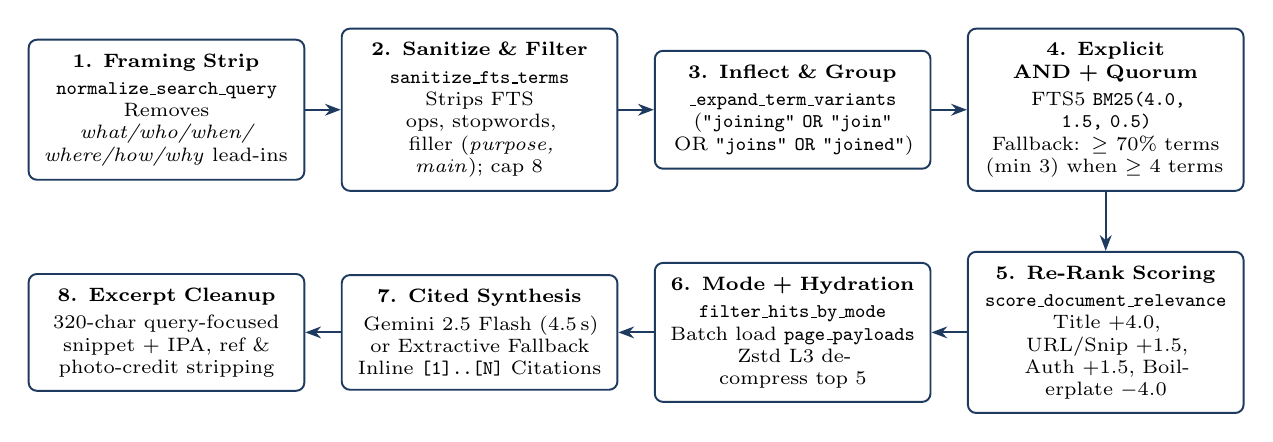
\begin{tikzpicture}[
    node distance=0.45cm and 0.45cm,
    snode/.style={
        rectangle, rounded corners=3pt, draw=NavyPrimary, fill=white,
        line width=0.7pt, text width=3.15cm, align=center, font=\scriptsize, inner sep=5pt
    },
    arr/.style={-{Stealth[length=2mm]}, line width=0.75pt, draw=NavyPrimary}
]
\node[snode] (s1) {\textbf{1. Framing Strip}\\[2pt]\texttt{normalize\_search\_query}\\Removes \textit{what/who/when/\\where/how/why} lead-ins};
\node[snode, right=of s1] (s2) {\textbf{2. Sanitize \& Filter}\\[2pt]\texttt{sanitize\_fts\_terms}\\Strips FTS ops, stopwords,\\filler (\textit{purpose, main}); cap 8};
\node[snode, right=of s2] (s3) {\textbf{3. Inflect \& Group}\\[2pt]\texttt{\_expand\_term\_variants}\\(\texttt{"joining" OR "join"}\\OR \texttt{"joins" OR "joined"})};
\node[snode, right=of s3] (s4) {\textbf{4. Explicit AND + Quorum}\\[2pt]FTS5 \texttt{BM25(4.0, 1.5, 0.5)}\\Fallback: $\ge 70\%$ terms\\(min 3) when $\ge 4$ terms};

\node[snode, below=0.75cm of s4] (s5) {\textbf{5. Re-Rank Scoring}\\[2pt]\texttt{score\_document\_relevance}\\Title $+4.0$, URL/Snip $+1.5$,\\Auth $+1.5$, Boilerplate $-4.0$};
\node[snode, left=of s5] (s6) {\textbf{6. Mode + Hydration}\\[2pt]\texttt{filter\_hits\_by\_mode}\\Batch load \texttt{page\_payloads}\\Zstd L3 decompress top 5};
\node[snode, left=of s6] (s7) {\textbf{7. Cited Synthesis}\\[2pt]Gemini 2.5 Flash (4.5\,s)\\or Extractive Fallback\\Inline \texttt{[1]..[N]} Citations};
\node[snode, left=of s7] (s8) {\textbf{8. Excerpt Cleanup}\\[2pt]320-char query-focused\\snippet + IPA, ref \&\\photo-credit stripping};

\draw[arr] (s1) -- (s2);
\draw[arr] (s2) -- (s3);
\draw[arr] (s3) -- (s4);
\draw[arr] (s4) -- (s5);
\draw[arr] (s5) -- (s6);
\draw[arr] (s6) -- (s7);
\draw[arr] (s7) -- (s8);
\end{tikzpicture}}
\caption{Low-Level Design: Query sanitization, FTS5 grouping, re-ranking, and synthesis pipeline.}
\label{fig:lld-ranking}
\end{figure}

In stage~3, parenthesized inflection groups are joined with explicit \texttt{\texttt{AND}} rather than implicit whitespace to satisfy SQLite FTS5 parser rules. \texttt{\_expand\_term\_variants} covers regular \texttt{-ing}, \texttt{-ies}, \texttt{-ed}, sibilant \texttt{-es} (\texttt{indexes} $\to$ \texttt{index}, \texttt{classes} $\to$ \texttt{class}), and plural \texttt{-s} forms. Stage~5 sorts candidates by \texttt{(matched\_terms, rel\_score, db\_score)} using host-boundary validation (\texttt{\_is\_authoritative\_host}) and penalizes generic repository template phrases when \texttt{mode != "code"}.

\subsection{Live Discovery, Parsing \& Bounded Deduplication}
\begin{enumerate}[leftmargin=1.4em, itemsep=3pt]
    \item \textbf{Two-Pass Domain Diversity (\texttt{discovery.py}):} Concurrently queries DuckDuckGo HTML, Wikipedia API, HackerNews Algolia, Reddit JSON, arXiv Atom, GitHub Search (plus optional Brave Search) excluding domains in the 24\,h WAF cooldown cache. Pass~1 selects at most \texttt{1} URL per domain; Pass~2 backfills remaining slots up to \texttt{max\_urls} from multi-article hubs (\texttt{en.wikipedia.org}, \texttt{arxiv.org}, \texttt{github.com}, \texttt{stackoverflow.com}).
    \item \textbf{Polite Chrome-Impersonated Fetch (\texttt{robots.py}, \texttt{parser.py}):} Fetches \texttt{robots.txt} per domain under an \texttt{asyncio.Lock} (24\,h TTL, supporting fractional \texttt{Crawl-delay}), then executes \texttt{curl\_cffi} (\texttt{impersonate="chrome124"}) capped at \texttt{12} concurrent fetches. \texttt{selectolax.lexbor} extracts \texttt{\_\_NEXT\_DATA\_\_} SSR JSON, Schema.org JSON-LD metadata, structured Markdown, and up to \texttt{max\_links=80} followable outbound links while filtering Cloudflare/Akamai challenge pages (\texttt{is\_waf\_or\_empty\_page}).
    \item \textbf{Deduplication \& Compression (\texttt{bloom.py}, \texttt{dedup.py}, \texttt{compression.py}):} A $10^6$-capacity \texttt{URLBloomFilter} (\texttt{mmh3} + \texttt{bitarray}, \texttt{0.1\%} FP rate) warms from \texttt{search\_index} at boot. Before saving, \texttt{compute\_simhash} hashes unigrams and 2-gram shingles over the leading \texttt{12,000} characters (\texttt{Hamming <= 3} per domain), avoiding multi-second CPU stalls on 2\,MB encyclopedia pages, and \texttt{zstd.ZstdCompressor(level=3)} compresses full Markdown into \texttt{page\_payloads}.
\end{enumerate}

% ==============================================================================
% SECTION 5: STORAGE MODEL
% ==============================================================================
\clearpage
\section{Storage Schema (\texttt{Turso LibSQL FTS5})}

All tables, FTS5 virtual indexes, synchronization triggers, compressed blobs, and crawl queues reside in one serverless Turso LibSQL database (\texttt{migrations/03\_turso\_fts5\_schema.sql}), illustrated in Figure~\ref{fig:erd}.

\begin{figure}[H]
\centering
\resizebox{0.95\textwidth}{!}{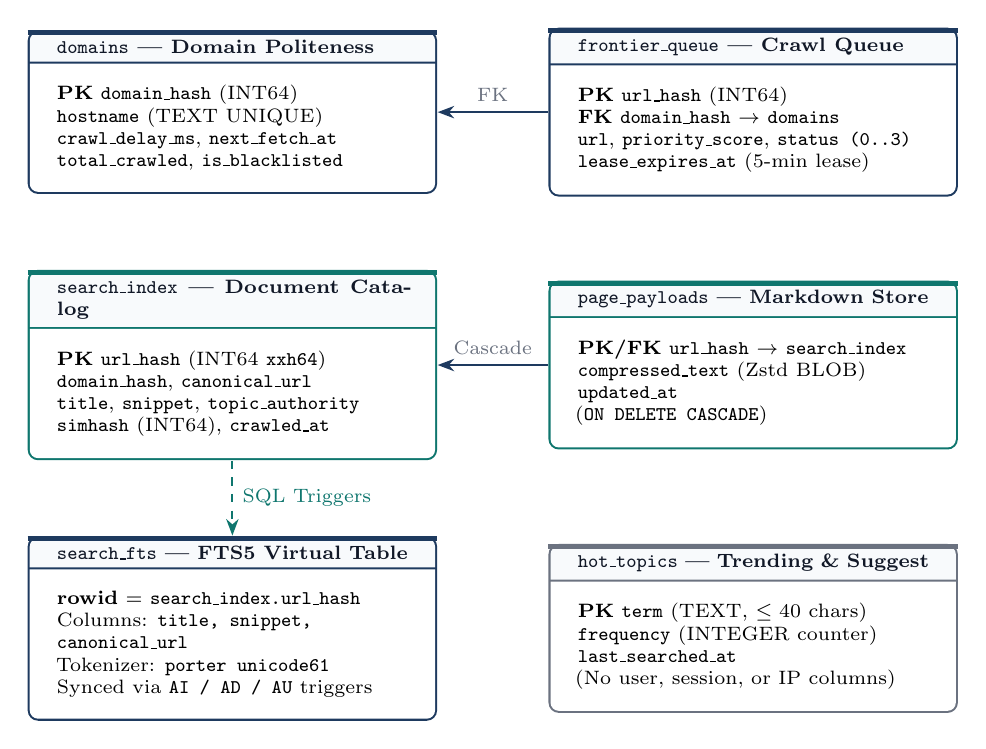
\begin{tikzpicture}[
    node distance=0.95cm and 1.4cm,
    arr/.style={-{Stealth[length=2.1mm]}, line width=0.75pt, draw=NavyPrimary},
    trig/.style={-{Stealth[length=2.1mm]}, dashed, line width=0.75pt, draw=TealAccent}
]

\newcommand{\erdbox}[3]{%
    \begin{tcolorbox}[enhanced, colback=white, colframe=#1, colbacktitle=SurfaceTint, coltitle=HeadingInk,
        fonttitle=\scriptsize\bfseries, title=#2, width=5.2cm, boxrule=0.75pt, arc=3pt,
        left=7pt, right=7pt, top=5pt, bottom=5pt, borderline north={1.8pt}{0pt}{#1}, nobeforeafter]
        \scriptsize\raggedright #3
    \end{tcolorbox}%
}

\node[inner sep=0pt] (domains) {\erdbox{NavyPrimary}{\texttt{domains} \textemdash{} Domain Politeness}{%
    \textbf{PK} \texttt{domain\_hash} (INT64)\\
    \texttt{hostname} (TEXT UNIQUE)\\
    \texttt{crawl\_delay\_ms}, \texttt{next\_fetch\_at}\\
    \texttt{total\_crawled}, \texttt{is\_blacklisted}%
}};

\node[inner sep=0pt, right=of domains] (frontier) {\erdbox{NavyPrimary}{\texttt{frontier\_queue} \textemdash{} Crawl Queue}{%
    \textbf{PK} \texttt{url\_hash} (INT64)\\
    \textbf{FK} \texttt{domain\_hash} $\to$ \texttt{domains}\\
    \texttt{url}, \texttt{priority\_score}, \texttt{status (0..3)}\\
    \texttt{lease\_expires\_at} (5-min lease)%
}};

\node[inner sep=0pt, below=of domains] (sindex) {\erdbox{TealAccent}{\texttt{search\_index} \textemdash{} Document Catalog}{%
    \textbf{PK} \texttt{url\_hash} (INT64 \texttt{xxh64})\\
    \texttt{domain\_hash}, \texttt{canonical\_url}\\
    \texttt{title}, \texttt{snippet}, \texttt{topic\_authority}\\
    \texttt{simhash} (INT64), \texttt{crawled\_at}%
}};

\node[inner sep=0pt, right=of sindex] (payloads) {\erdbox{TealAccent}{\texttt{page\_payloads} \textemdash{} Markdown Store}{%
    \textbf{PK/FK} \texttt{url\_hash} $\to$ \texttt{search\_index}\\
    \texttt{compressed\_text} (Zstd BLOB)\\
    \texttt{updated\_at}\\
    (\texttt{ON DELETE CASCADE})%
}};

\node[inner sep=0pt, below=of sindex] (fts) {\erdbox{NavyPrimary}{\texttt{search\_fts} \textemdash{} FTS5 Virtual Table}{%
    \textbf{rowid} = \texttt{search\_index.url\_hash}\\
    Columns: \texttt{title, snippet, canonical\_url}\\
    Tokenizer: \texttt{porter unicode61}\\
    Synced via \texttt{AI / AD / AU} triggers%
}};

\node[inner sep=0pt, right=of fts] (hot) {\erdbox{MutedInk}{\texttt{hot\_topics} \textemdash{} Trending \& Suggest}{%
    \textbf{PK} \texttt{term} (TEXT, $\le 40$ chars)\\
    \texttt{frequency} (INTEGER counter)\\
    \texttt{last\_searched\_at}\\
    (No user, session, or IP columns)%
}};

\draw[arr] (frontier.west) -- node[above, font=\scriptsize\color{MutedInk}] {FK} (domains.east);
\draw[arr] (payloads.west) -- node[above, font=\scriptsize\color{MutedInk}] {Cascade} (sindex.east);
\draw[trig] (sindex.south) -- node[right, font=\scriptsize\color{TealAccent}] {SQL Triggers} (fts.north);

\end{tikzpicture}}
\caption{Turso LibSQL relational and FTS5 schema (\texttt{migrations/03\_turso\_fts5\_schema.sql}).}
\label{fig:erd}
\end{figure}

% ==============================================================================
% SECTION 6: AI RETRIEVAL & EXA AGENT INTERFACE
% ==============================================================================
\section{AI Retrieval Engine \& Exa-Compatible Agent Interface}

To support autonomous AI agents (\textit{e.g.}, LangChain \texttt{ExaSearchRetriever}, LlamaIndex, AutoGen, and custom ReAct loops), Neutron v3.0 provides full protocol parity with the Exa.ai API, enabling zero-configuration drop-in replacement via the official \texttt{exa-py} SDK.

\subsection{Heuristic Intent Routing (\texttt{classify\_query\_intent})}
Modern search workloads bifurcate into two retrieval paradigms: exact lexical lookups (\textit{e.g.}, function signatures, error codes, quoted terms) and semantic exploration (\textit{e.g.}, conversational queries, conceptual comparisons, open-ended research). Neutron implements a smart heuristic classifier that routes requests dynamically:
\begin{itemize}
    \item \textbf{\texttt{keyword}}: Selected for quoted phrases (\texttt{"..."}), code symbols (\texttt{\_}, \texttt{()}, \texttt{->}, \texttt{::}), camelCase identifiers, domain prefixes (\texttt{site:}, \texttt{filetype:}), and 1--2 token queries. Queries execute against Porter-stemmed FTS5 BM25 with quorum fallback.
    \item \textbf{\texttt{neural}}: Selected for conversational questions (\textit{who}, \textit{what}, \textit{when}, \textit{where}, \textit{how}, \textit{why}), comparison operators (\textit{vs}, \textit{difference}), recommendation phrases (\textit{best}, \textit{guide}), or multi-term natural language queries. Triggers query expansion, live web discovery adapters, and cited synthesis.
\end{itemize}

\subsection{Exa Drop-In Endpoints \& Entity Dossier Traversal}
The Edge Gateway exposes the complete Exa API contract over standard HTTPS JSON:
\begin{itemize}
    \item \textbf{\texttt{POST /search}}: Accepts Exa payloads (\texttt{query}, \texttt{type}, \texttt{numResults}, \texttt{category}, \texttt{contents}, \texttt{subpages}, \texttt{livecrawl}), returning \texttt{resolvedSearchType}, ranked results with clean Markdown, snippet highlights, subpages, and optional grounded answers.
    \item \textbf{\texttt{POST /contents}}: Batch extracts clean Markdown, entity highlights, and child subpages for up to 20 target URLs in a single round-trip, leveraging the compressed \texttt{page\_payloads} store.
    \item \textbf{\texttt{POST /findSimilar}}: Discovers structurally and topically related URLs from a seed document, computing SimHash Hamming distances and cross-domain keyword clusters while excluding the source domain.
    \item \textbf{Subpage Dossiers}: The parser extracts candidate internal links matching priority documentation paths (\texttt{docs/}, \texttt{api/}, \texttt{pricing/}, \texttt{guides/}) and hydates child documents directly into the response entity tree.
\end{itemize}

% ==============================================================================
% SECTION 7: BUDGETS, SECURITY & VERIFICATION
% ==============================================================================
\clearpage
\section{Latency Budgets, Security Controls \& Tooling}

Figure~\ref{fig:latency-budgets} summarizes the configured stage budgets defined in \texttt{services/common/config.py}. Tight per-fetch (\texttt{3.5\,s}), Gemini (\texttt{4.5\,s}), and JIT batch (\texttt{8.5\,s}) ceilings keep streaming responses interactive while still completing Turso writes on free-tier compute.

\begin{figure}[H]
\centering
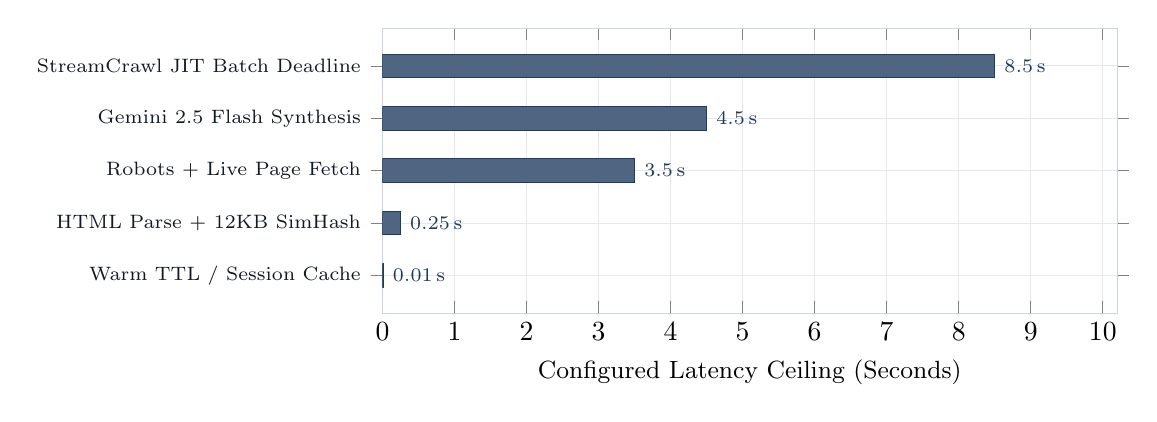
\begin{tikzpicture}
\begin{axis}[
    xbar,
    width=0.90\textwidth,
    height=5.2cm,
    bar width=8.5pt,
    xmin=0, xmax=10.2,
    xlabel={\small Configured Latency Ceiling (Seconds)},
    symbolic y coords={
        Warm TTL / Session Cache,
        HTML Parse + 12KB SimHash,
        Robots + Live Page Fetch,
        Gemini 2.5 Flash Synthesis,
        StreamCrawl JIT Batch Deadline
    },
    ytick=data,
    yticklabel style={font=\scriptsize\color{HeadingInk}},
    nodes near coords={\pgfmathprintnumber[fixed,precision=2]{\pgfplotspointmeta}\,s},
    nodes near coords style={font=\scriptsize\color{NavyPrimary}},
    nodes near coords align={horizontal},
    grid=major,
    major grid style={LightRule},
    axis line style={BorderGray},
    enlarge y limits=0.18
]
\addplot[fill=NavyPrimary!78!white, draw=NavyPrimary] coordinates {
    (0.01,Warm TTL / Session Cache)
    (0.25,HTML Parse + 12KB SimHash)
    (3.50,Robots + Live Page Fetch)
    (4.50,Gemini 2.5 Flash Synthesis)
    (8.50,StreamCrawl JIT Batch Deadline)
};
\end{axis}
\end{tikzpicture}
\caption{Configured latency envelopes across cache, crawl, and synthesis tiers.}
\label{fig:latency-budgets}
\end{figure}

\begin{table}[H]
\centering
\small
\renewcommand{\arraystretch}{1.28}
\begin{tabularx}{\textwidth}{@{}>{\ttfamily\scriptsize\color{NavyPrimary}\raggedright\arraybackslash}p{5.4cm} >{\raggedright\arraybackslash}X@{}}
\toprule
\textbf{Workflow / Utility} & \textbf{Function} \\
\midrule
.github/workflows/ci\_cd.yml &
Runs \texttt{compileall}, \texttt{ruff check --select E9,F63,F7,F82,F401}, Vite frontend build (\texttt{tsc -b \&\& vite build}), \texttt{44} unit/integration tests, and Turso schema migration. \\
.github/workflows/deploy\_pages.yml &
Builds \texttt{frontend/} targeting \texttt{VITE\_API\_BASE\_URL} (\texttt{https://neutron-gateway.onrender.com}) and publishes static bundles and PDF docs to GitHub Pages. \\
scripts/gen\_proto.py &
Regenerates Python ConnectRPC and Protobuf stubs from \texttt{proto/neutron/v1/neutron.proto}. \\
scripts/refresh\_stale.py &
Queries oldest \texttt{search\_index} rows (\texttt{row.asdict()}), verifies \texttt{robots.txt} and \texttt{text/html}, and updates Markdown payloads with full \texttt{1,200}-char snippets. \\
\bottomrule
\end{tabularx}
\caption{Continuous integration workflows and maintenance utilities.}
\end{table}

\begin{designnote}[Privacy \& Frontend Security Summary]
\begin{itemize}[leftmargin=1.2em, itemsep=2pt]
    \item Rate limiting (\texttt{30/min} \texttt{/search}, \texttt{15/min} \texttt{/search/stream}, \texttt{20/min} \texttt{/api/research}) uses volatile in-memory \texttt{X-Forwarded-For} buckets and sets \texttt{X-Content-Type-Options: nosniff}, \texttt{Referrer-Policy: no-referrer}, and \texttt{Permissions-Policy: interest-cohort=()}.
    \item Search snippets render strictly via React text nodes and \texttt{<mark>} spans (no \texttt{dangerouslySetInnerHTML}); Reader Markdown passes through \texttt{marked} + \texttt{DOMPurify} (\texttt{ALLOWED\_URI\_REGEXP: \^{}https?://}); and outbound anchors are filtered with \texttt{safeHttpUrl}.
\end{itemize}
\end{designnote}

\end{document}
